\section{Introduction}
\label{network:ntlm:authentication}
LM and  NTLM here are the hash names, and NTLMv1 and NTLMv2 are authentication  protocols that utilize the LM or NT hash. Below is a quick comparison  between these hashes and protocols, which shows us that, while not  perfect by any means, Kerberos is often the authentication protocol of  choice wherever possible. It is essential to understand the difference  between the hash types and the protocols that use them.

\begin{tabular}{|l|l|l|l|l|}
 \hline \hline
 Hash     & Crypto    & Mutual & Msg Type & Trusted  \\
 Protocol & technique &  Authn &          & 3d Party \\
 \hline \hline
 NTLM & Sym  & No & Rnd nbr & DC \\
 NTLMv1 & Sym  & No & MD4 hash, rnd nbr & DC \\
 NTLMv2 & Sym  & No & MD4 hash, rnd nbr & DC \\
 Kerberos & Sym \& Asym & Yes & Encrypted ticket using DES, MD5 & DC, KDC \\
 \hline \hline
\end{tabular}

\subsection{Hashes}
\subsubsection{LM}

LAN Manager (LM) hashes are the oldest password storage Windows operating system. Due to significant security weaknesses in the hashing  algorithm it has been turned off by default since  Windows Vista/Server 2008. However, it is still common to encounter,  especially in large environments where older systems are still used.  Passwords using LM are limited to a maximum of 14  characters. Passwords are not case sensitive and are converted to  uppercase before generating the hashed value, limiting the keyspace to a  total of 69 characters making it relatively easy to crack these hashes  using a tool such as Hashcat.

An LM hash takes the form of \verb+299bd128c1101fd6+.


{\bf LMOWFv1} (implemented in the \href{https://github.com/fortra/impacket/blob/9a8d27034eab20d23802730d0c69bf99356d8af1/impacket/ntlm.py#L742C1-L747}{compute\_lmhash function}),  used only by LM and NTLMv1, is an NT LAN Manager (LM) one-way function that creates a hash based on the user's password to generate a principal's security key. 

{\bf LMOWFv2} (implemented in the \href{https://github.com/fortra/impacket/blob/9a8d27034eab20d23802730d0c69bf99356d8af1/impacket/ntlm.py#L896C1-L897}{LMOWFv2 function}) Based on The LAN Manager (LM) version 2, a one-way function (OWF) used to create a hash based on the user's password to generate a principal's secret key

\subsubsection{NTHash (NTLM)}

These hashes are stored locally in the SAM database or the \gls{win:NTDS.DIT}
database file on a Domain Controller. The protocol has two hashed  password
values to choose from to perform authentication: the LM hash (as discussed
above) and the NT hash, which is the MD4 hash of the little-endian UTF-16 value
of the password.

Even though they are considerably stronger than LM hashes (supporting the entire Unicode character set of 65,536 characters), they can still  be brute-forced offline relatively quickly using a tool such as Hashcat. NTLM is also vulnerable to the  pass-the-hash attack.

An NTLM hash looks like this:

\begin{verbatim}
Rachel:500:aad3c435b514a4eeaad3b935b51304fe:e46b9e548fa0d122de7f59fb6d48eaa2:::
\end{verbatim}

Looking at the hash above, we can break the NTLM hash down into its individual parts:
\begin{itemize}
    \item  \verb+Rachel+ is the username
    \item  \verb+500+ is the Relative Identifier (RID). 500 is the known RID for the administrator account
    \item  \verb+aad3c435b514a4eeaad3b935b51304fe+ is the LM hash and, if LM hashes are disabled on the system, can not be used for anything
    \item  \verb+e46b9e548fa0d122de7f59fb6d48eaa2+ is the NT hash. This hash can either be cracked offline or used for a pass-the-hash attack.
\end{itemize}

{\bf NTOWFv1} (used only by NTLMv1 and implemented in the \href{https://github.com/fortra/impacket/blob/9a8d27034eab20d23802730d0c69bf99356d8af1/impacket/ntlm.py#L759-L769}{compute\_nthash} function), is an NT LAN Manager (NT) one-way function that creates a hash based on the user's password to generate a principal's security key:

{\bf NTOWFv2} (implemented in the \href{https://github.com/fortra/impacket/blob/9a8d27034eab20d23802730d0c69bf99356d8af1/impacket/ntlm.py#L889C1-L894}{NTOWFv2 function}) Based on the NT LAN Manager (NTLM) (NT) version 2, a one-way function (OWF) used to create a hash based on the user's password to generate a principal's secret key.


\subsubsection{Domain Cached Credentials (MSCache2)}
In an AD environment, the authentication methods require the host we are trying to access to  communicate with the Domain Controller.  Microsoft developed the MS Cache v1 and v2 algorithm (also known as Domain Cached Credentials  (DCC) to solve the potential issue of a domain-joined host being unableto communicate with a domain controller.

Hosts save the last ten hashes for any domain users that successfully log into the machine in the \verb+HKEY_LOCAL_MACHINE\SECURITY\Cache+  registry key. These hashes cannot be used in pass-the-hash attacks.  Furthermore, the hash is very slow to crack.  

These hashes can be obtained by an attacker or pentester after gaining local admin access to a host and have thefollowing format:
\begin{verbatim}
$DCC2$10240#bjones#e4e938d12fe5974dc42a90120bd9c90f
\end{verbatim}



\subsection{Protocols}

NT Lan Manager (NTLM/MS-NLMP) is the name of a family of security protocols (LM, NTLMv1, and NTLMv2) used by application protocols to authenticate remote users and optionally provide session security when requested by the application.

The NTLM security protocols are all embedded protocols, meaning that although NTLM has messages and a state machine like other protocols, it does not have a network protocol stack layer. This nature of NTLM allows any protocol with a defined layer in the network stack (such as SMB, HTTP(S), and LDAP(S)) to utilize it.

NTLM is a challenge-response protocol that uses nonces, pseudo-random numbers generated for one-time use, as a defensive mechanism against replaying attacks.

Each protocol has two variants, connection-oriented and connectionless.

\begin{itemize}
    \item 
        Security Support Provider Interface (SSPI) is an API that allows connected applications to call one of several security providers to establish authenticated connections and to exchange data securely over those connections.
    \item  
        A security support provider (SSP) is a dynamic-link library (DLL) responsible for implementing the SSPI by exposing one or more security packages to applications; each security package provides mappings between an application's SSPI function calls and an actual security model's functions. 
    \item 
        NTLM SSP (\verb+%Windir%\System32\msv1_0.dll+) is a binary messaging protocol utilized by SSPI to facilitate NTLM challenge-response authentication and to negotiate options for integrity and confidentiality
\end{itemize}

Both domain-joined and workgroup computers can utilize NTLM for authentication

always keep in mind the following:
\begin{itemize}
    \item 
        The NTLM version used on hosts, whether NTLMv1 or NTLMv2, is \href{https://learn.microsoft.com/en-us/windows/security/threat-protection/security-policy-settings/network-security-lan-manager-authentication-level}{configured out-of-band} before authentication.
    \item
        Using a secure mechanism, the client and server/DC share a secret key (the user's password's hash) before authentication.
    \item
        Neither plaintext credentials nor the shared secret key are sent over the wire.
\end{itemize}


\subsection{Authentication Workflow}

NT LAN Manager (NTLM)  is a
challenge-response authentication protocol and uses  three messages to
authenticate: 
\begin{enumerate}
    \item {\bf Negotiate} a client first sends a
        \href{https://docs.microsoft.com/en-us/openspecs/windows_protocols/ms-nlmp/b34032e5-3aae-4bc6-84c3-c6d80eadf7f2}{NEGOTIATE\_MESSAGE} ({\bf Type 1 message}) to the server
    \item {\bf Challenge} the server sends a \href{https://docs.microsoft.com/en-us/openspecs/windows_protocols/ms-nlmp/801a4681-8809-4be9-ab0d-61dcfe762786}{CHALLENGE\_MESSAGE} ({\bf Type 2 message}) to the client. This is nothing more than a 64-bit random value that changes with each authentication request .
    \item {\bf Response} The client send a \href{https://docs.microsoft.com/en-us/openspecs/windows_protocols/ms-nlmp/033d32cc-88f9-4483-9bf2-b273055038ce}{AUTHENTICATE\_MESSAGE} (\bf Tpe3 message) which contains the encrypted challenge (using a hashed version of its password as the key),  its username and possibly its domain
        \end{enumerate}

\begin{figure}[!ht]
  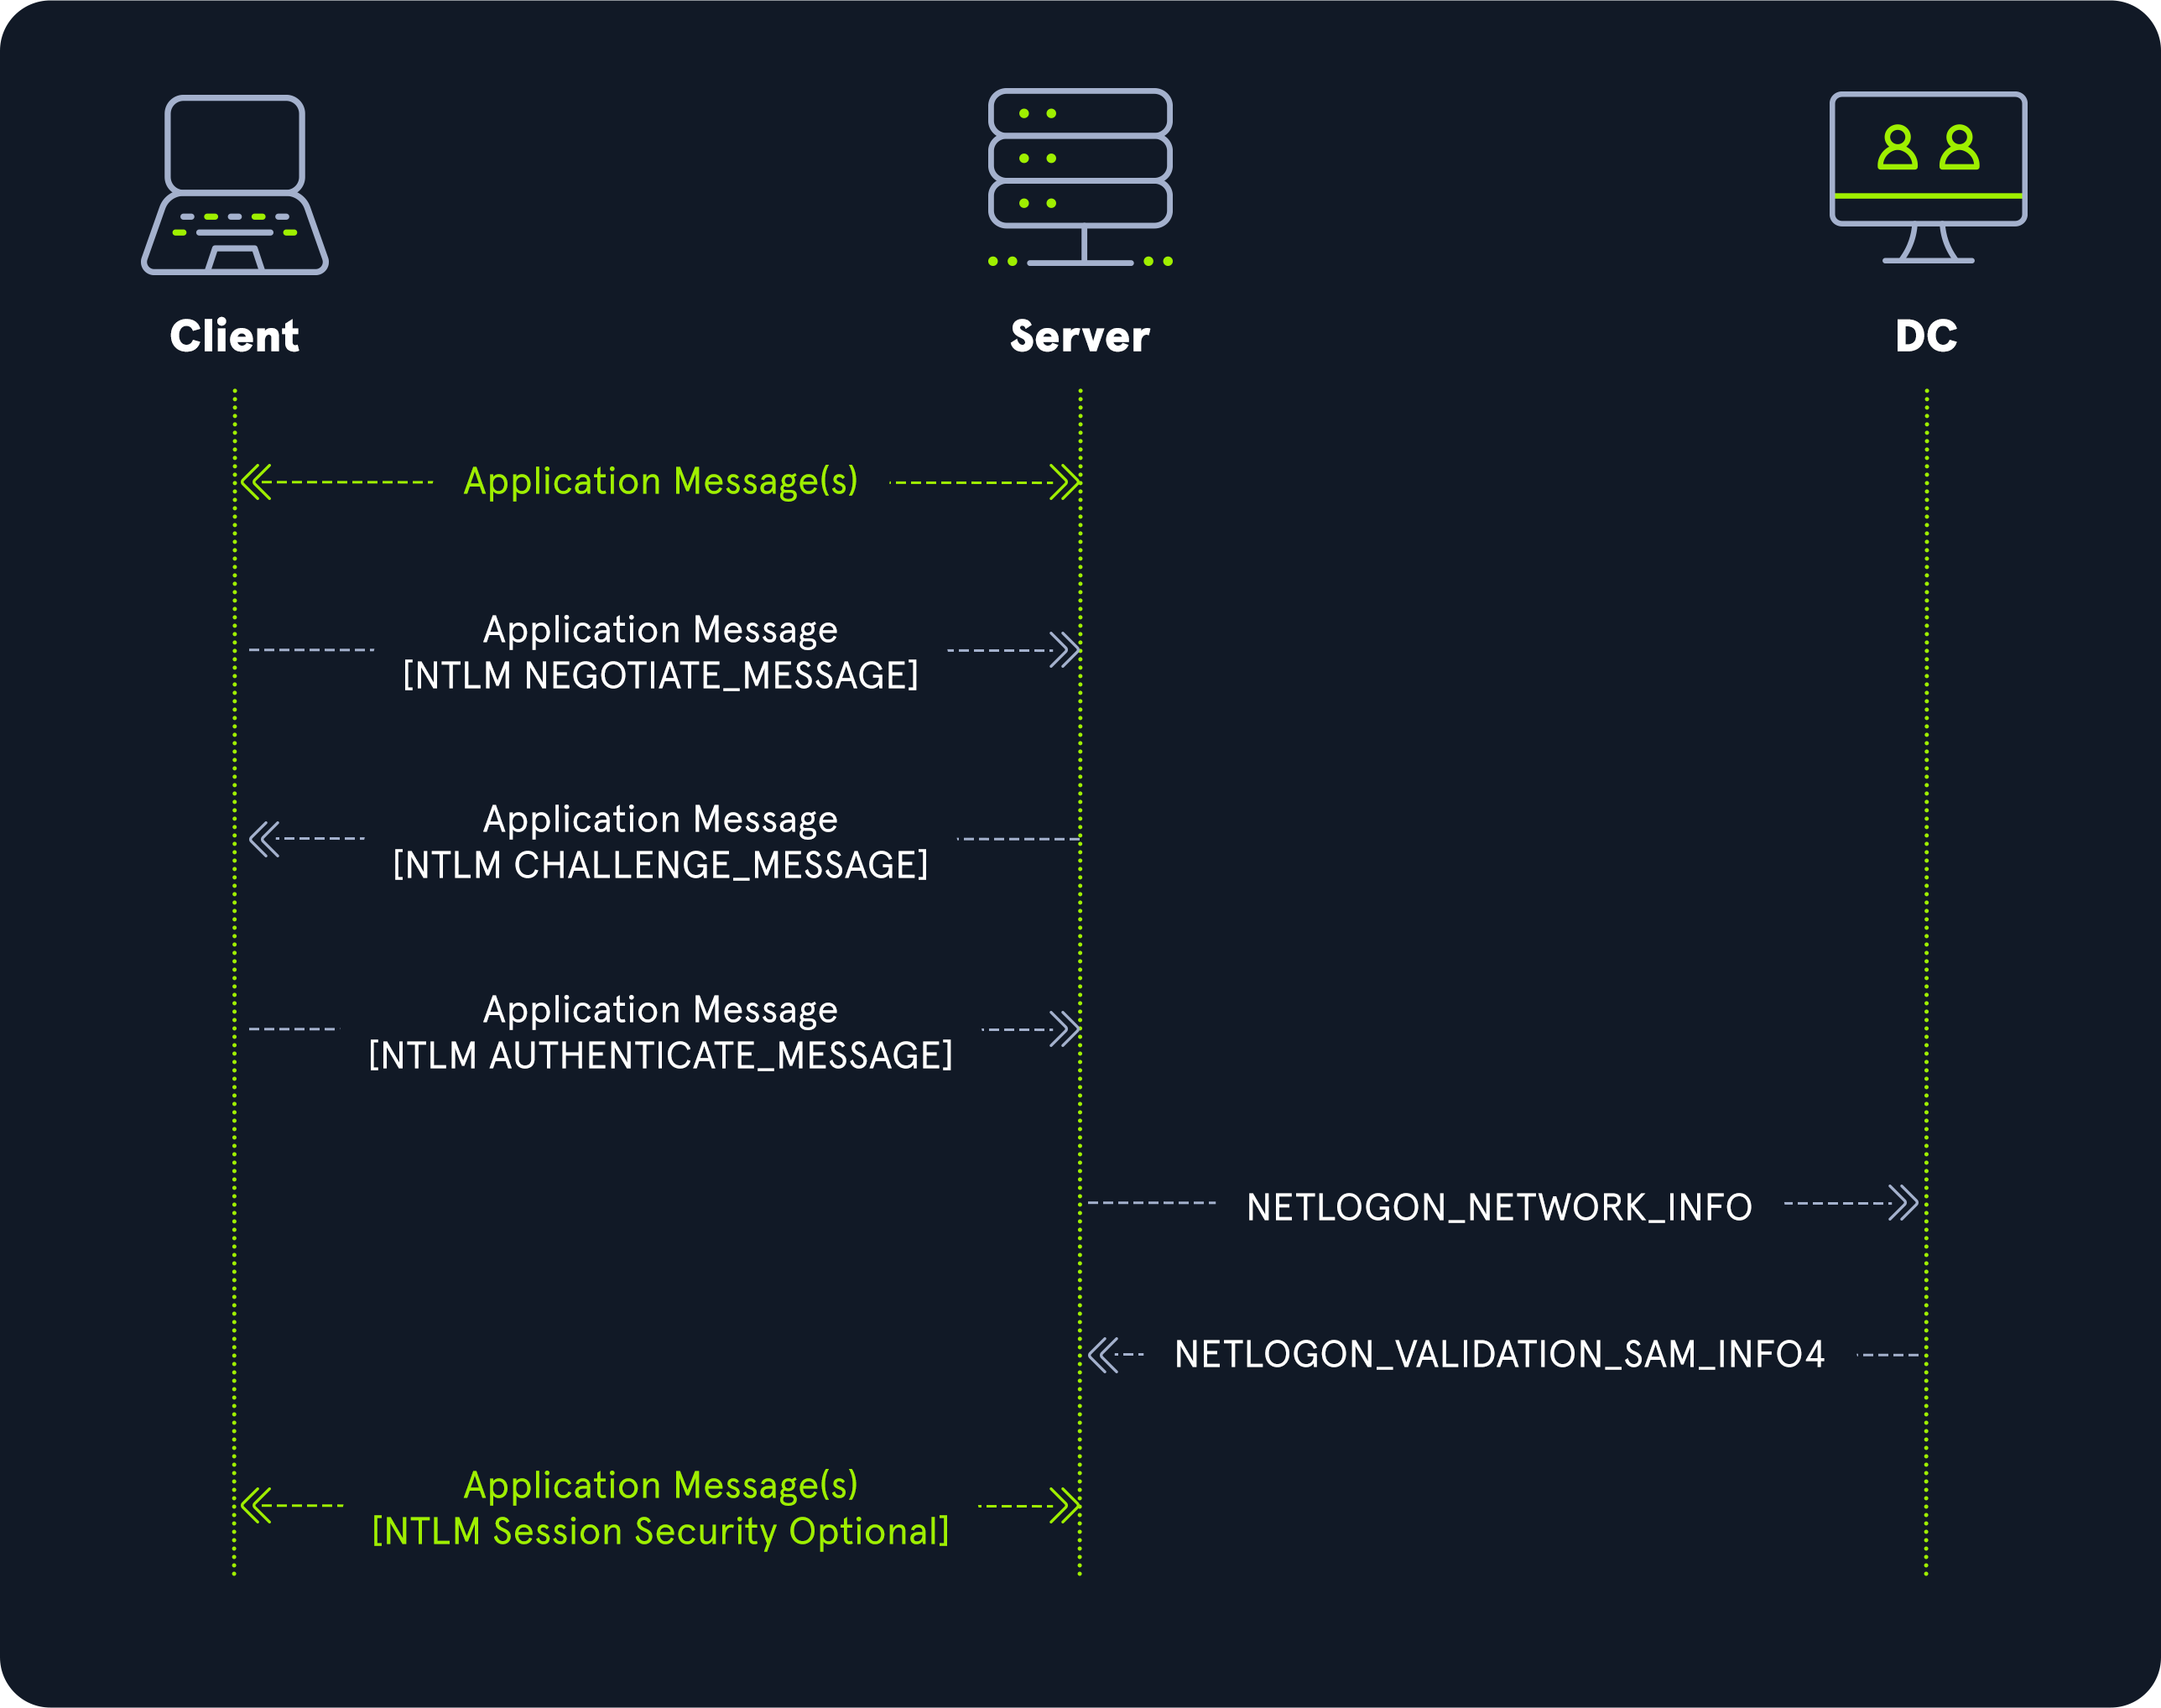
\includegraphics[width=\linewidth]{network/ntlm/images/Domain-joined_Computers_NTLM_Authentication.png}
  \caption{Domain joined NTLM protocol}
  \label{fig:domain-ntlm-protocol}
\end{figure}

\begin{figure}[!ht]
  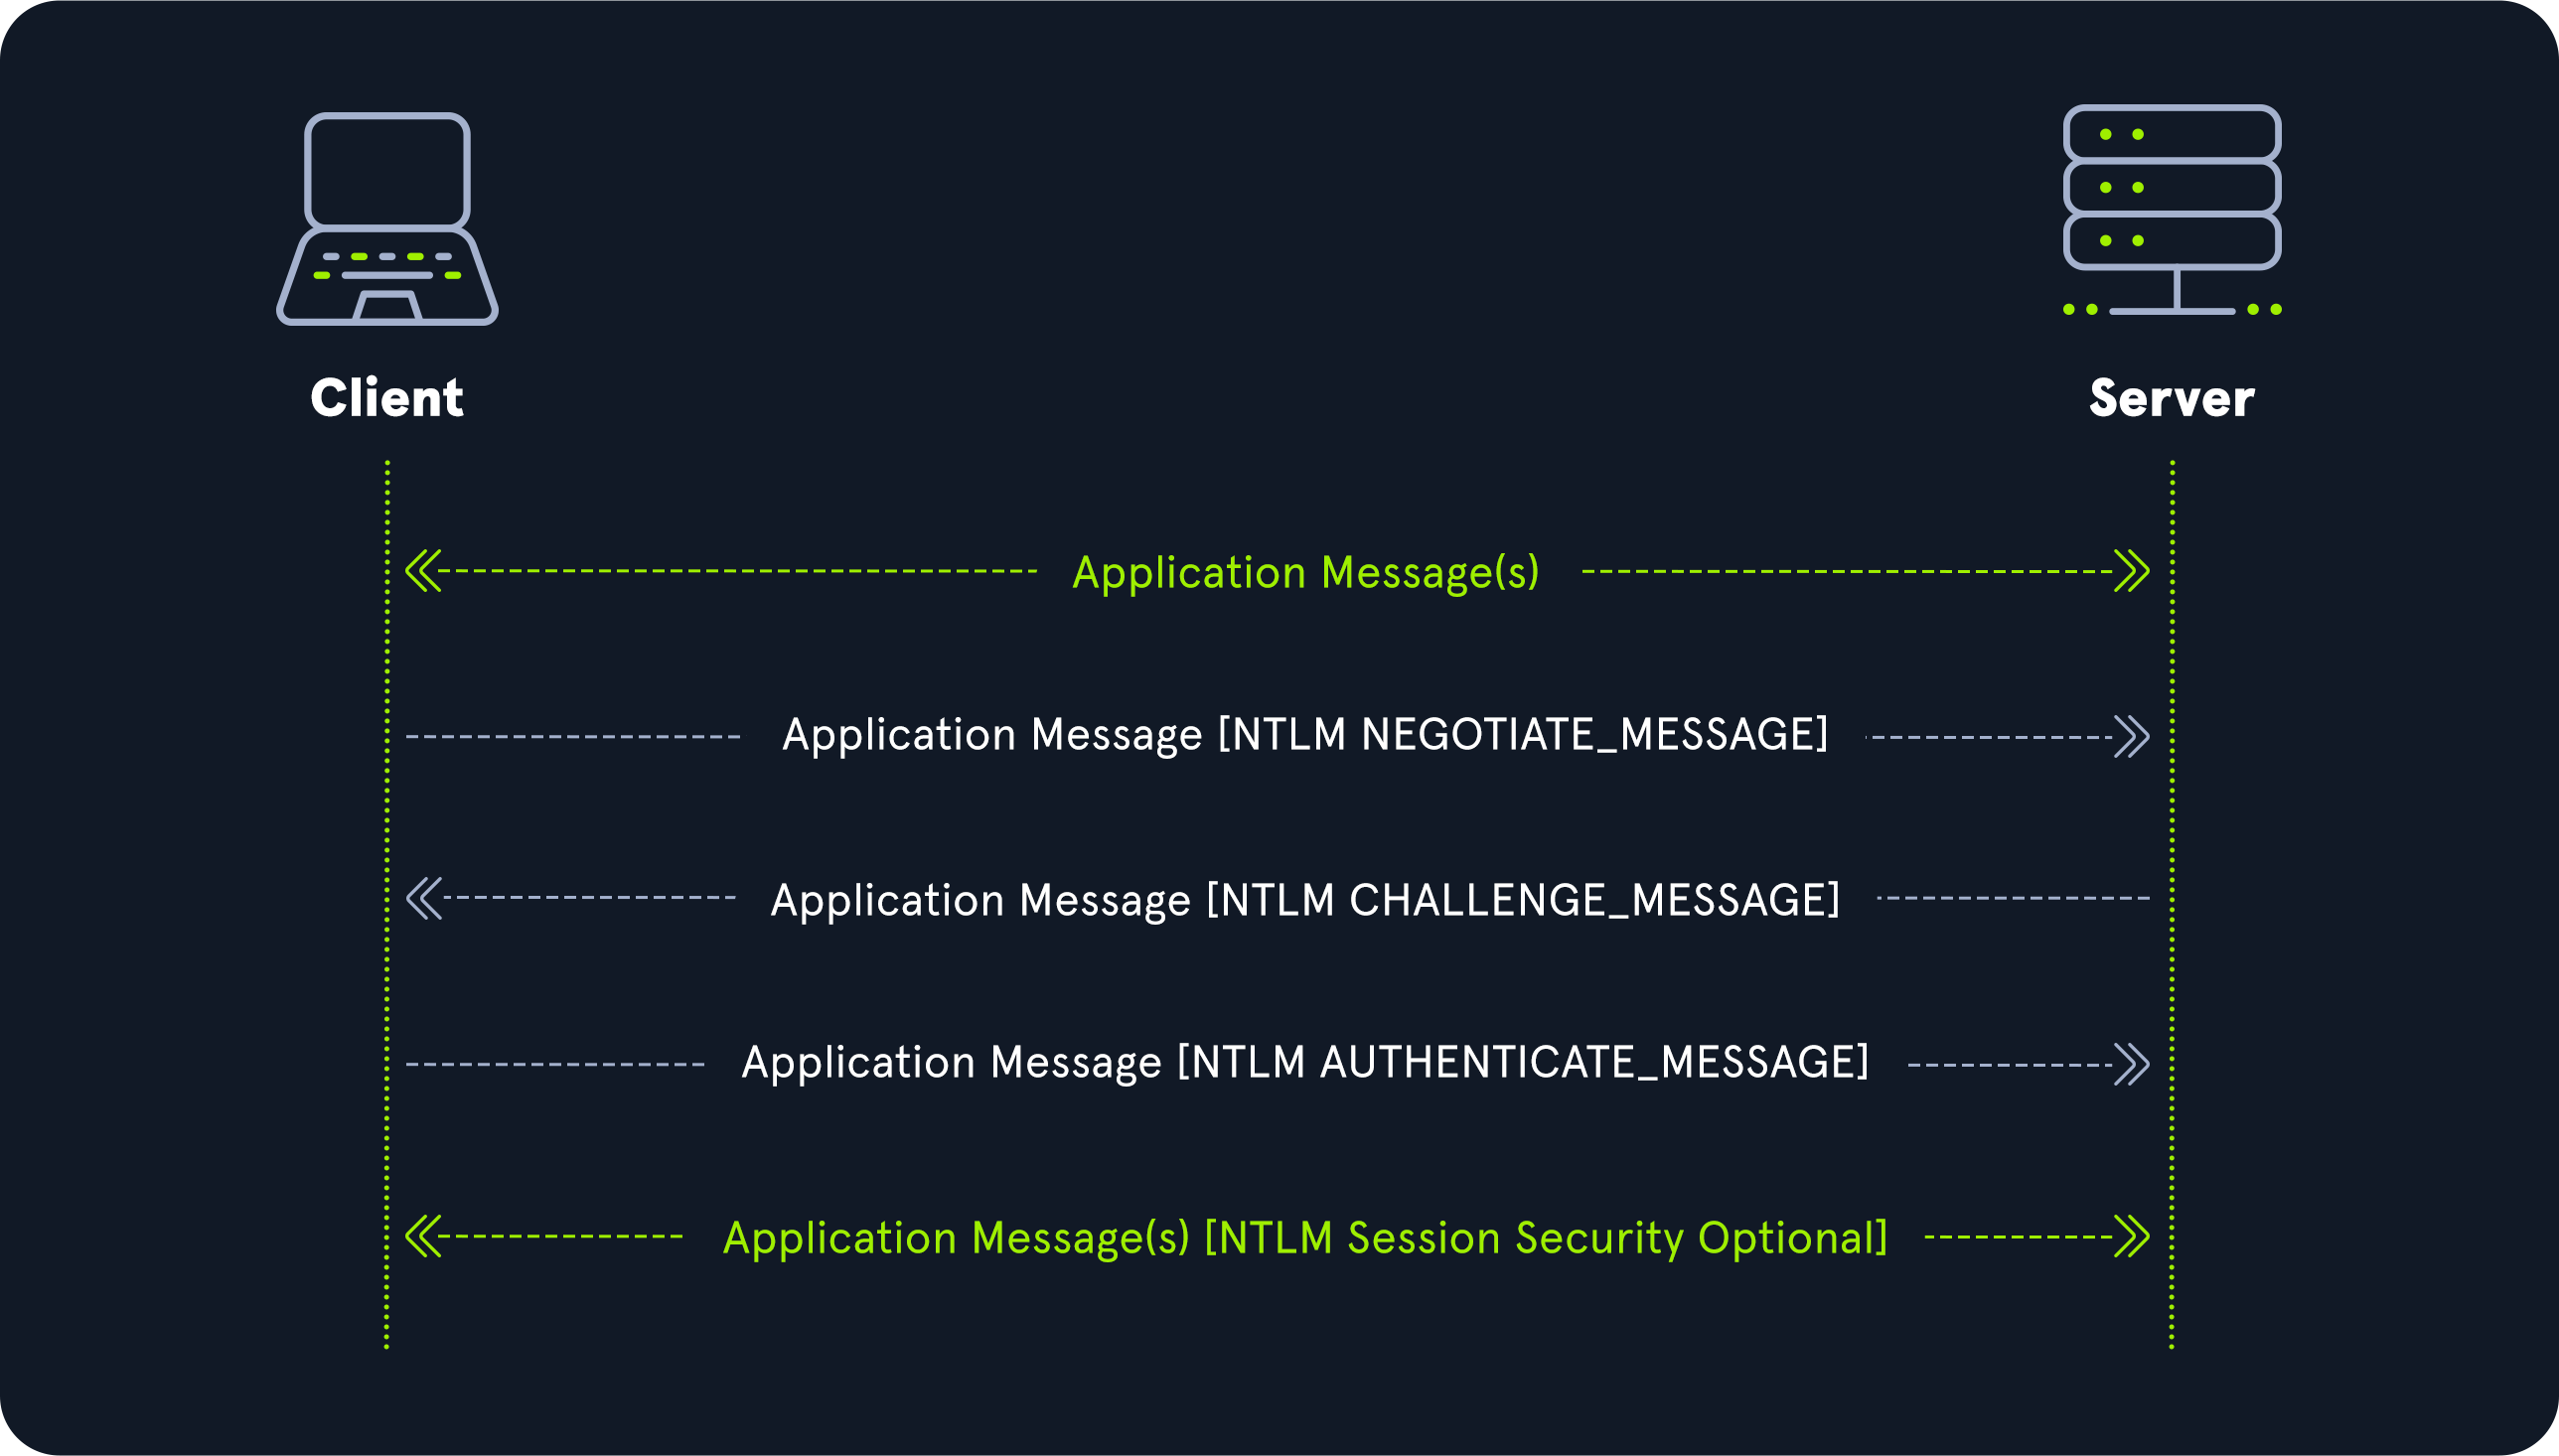
\includegraphics[width=\linewidth]{network/ntlm/images/Workgroup_Computers_NTLM_Authentication.png}
  \caption{Workgroup NTLM protocol}
  \label{fig:workgroup-ntlm-protocol}
\end{figure}

Once it receives the \verb+AUTHENTICATE_MESSAGE+, and because it does not possess the client's secret key, the server delegates the verification of the user's identity to a DC (a procedure known as \href{https://learn.microsoft.com/en-us/openspecs/windows_protocols/ms-nrpc/70697480-f285-4836-9ca7-7bb52f18c6af}{Pass-through authentication}) by invoking \href{https://learn.microsoft.com/en-us/openspecs/windows_protocols/ms-nrpc/d17f1077-de4b-4fcd-8867-39068cb789f5}{NetrLogonSamLogonWithFlags}, which contains \href{https://learn.microsoft.com/en-us/openspecs/windows_protocols/ms-nrpc/e17b03b8-c1d2-43a1-98db-cf8d05b9c6a8}{NETLOGON\_NETWORK\_INFO}, a data structure populated with the various fields that the DC requires to verify the user.

If authentication is successful, the DC returns a \href{https://learn.microsoft.com/en-us/openspecs/windows_protocols/ms-nrpc/bccfdba9-0c38-485e-b751-d4de1935781d}{NETLOGON\_VALIDATION\_SAM\_INFO4} data structure to the server, and the server establishes an authenticated session with the client; otherwise, the DC returns an error, and the server might return an error message to the client, or, it can simply terminate the connection.

\subsection{NTLM Messages}

Each NTLM message is variable-length, containing a:
\begin{itemize}
    \item 
        fixed-length {\bf header} which contains in order:
        \begin{itemize}
            \item the signature: 8-byte NULL-terminated ASCII string always set to \verb+[N, T, L, M, S, S, P, \0]+.
            \item the message type: 4-byte unsigned integer (\verb+0x00000001 = NtLmNegotiate+, \verb+0x00000002=NtLmChallenge+, \verb+0x00000003=NtLmAuthenticate+ ) 
            \item MessageDependentFields: A variable-length field that contains the NTLM message contents.
        \end{itemize}
    \item 
        a variable-sized message {\bf payload}: contains a message-dependent number of individual payload messages, referenced by byte offsets in {\bf MessageDependentFields}.
\end{itemize}

\subsubsection{NEGOTIATE\_MESSAGE}

It contains four message-dependent fixed-length fields. One important field to know about is \verb+NegotiateFlags+. this 4-bytes field, present in all three NTLM messages and not exclusive to \verb+NEGOTIATE_MESSAGE+, is a \href{https://learn.microsoft.com/en-us/openspecs/windows_protocols/ms-nlmp/99d90ff4-957f-4c8a-80e4-5bfe5a9a9832}{NEGOTIATE} structure consisting of 32 1-bit flags that allow indicating which NTLM capabilities are supported/requested by the sender.

\subsubsection{CHALLENGE\_MESSAGE}

It contains six message-dependent fixed-length fields, two important:
\begin{itemize}
    \item 
        NegotiateFlags: holds the flags the server has chosen from the options offered/requested by the client in \verb+NegotiateFlags+ of the \verb+NEGOTIATE_MESSAGE+
    \item
        ServerChallenge: a 64-bit nonce that holds the NTLM challenge generated by the server.
\end{itemize}

Tools, such as \href{https://github.com/nopfor/ntlm_challenger}{NTLM Challenger}, \href{https://gitlab.com/Zer1t0/ntlm-info}{ntlm-info}, \href{https://github.com/praetorian-inc/NTLMRecon}{NTLMRecon}, and \href{https://github.com/fortra/impacket/blob/impacket_0_11_0/examples/DumpNTLMInfo.py}{DumpNTLMInfo.py} perform reconnaissance against endpoints/hosts that accept NTLM authentication by parsing the information returned within the \verb+CHALLENGE_MESSAGE+

\subsubsection{AUTHENTICATE\_MESSAGE}

It contains nine message-dependent fixed-length fields, three important to know about, 
\begin{itemize}
    \item 
        \verb+ClientChallenge+: The 8-byte challenge message generated by the client.
    \item 
        \verb+LmChallengeResponseFields+
    \item
        \verb+NtChallengeResponseFields+
\end{itemize}


\subsection{Protocol version and message calculation}

The NTLM protocol performs a challenge/response between a server and  client using the NT hash.

\subsubsection{NTLMv1 (Net-NTMLv1)}

If \verb+NTLMSSP_NEGOTIATE_LM_KEY+ (\verb+G+ bit of \verb+NEGOCIATE+) was agreed upon by the server and client in \verb+NegotiateFlags+ then:
\begin{itemize}
    \item 
        \verb+LmChallengeResponseFields+ contains a \href{https://learn.microsoft.com/en-us/openspecs/windows_protocols/ms-nlmp/e3fee6d1-0d93-4020-84ab-ca4dc5405fc9}{LM\_RESPONSE} structure
    \item
        \verb+NtChallengeResponseFields+ contains a \href{https://learn.microsoft.com/en-us/openspecs/windows_protocols/ms-nlmp/b88739c6-1266-49f7-9d22-b13923bd8d66}{NTLM\_RESPONSE} structure;
\end{itemize}

\verb+LM_RESPONSE+ contains one field, which is \verb+Response+, a 24-byte array of unsigned char that contains the client's \verb+LmChallengeResponse+

\verb+NTLM_RESPONSE+ contains one field, which is \verb+Response+, a 24-byte array of unsigned char that contains the client's \verb+NtChallengeResponse+

\href{https://learn.microsoft.com/en-us/openspecs/windows_protocols/ms-nlmp/464551a8-9fc4-428e-b3d3-bc5bfb2e73a5} {NTLM v1 Authentication pseudo-code} is implemented in \href{https://github.com/fortra/impacket/blob/9a8d27034eab20d23802730d0c69bf99356d8af1/impacket/ntlm.py#L717-L740}{computeResponseNTLMv1}

The algorithm  looks as follows:
\begin{verbatim}
C = 8-byte server challenge, random
K1 | K2 | K3 = LM/NT-hash | 5-bytes-0
response = DES(K1,C) | DES(K2,C) | DES(K3,C)
\end{verbatim}

Here's an example of a NTLMv2 hash:
\begin{verbatim}
Support1::WIN-OLMHXGAP0V2:e2dL3196O8f55fB6:Q49S19A2937J6XC3CKA418EI4958OHB9:xF2K324O5L6Q7V8C
\end{verbatim}



\subsubsection{NTLMv2 (Net-NTLMv2)}

If \verb+NTLMSSP_NEGOTIATE_LM_KEY+ (\verb+G+ bit of \verb+NEGOCIATE+) was agreed upon by the server and client in \verb+NegotiateFlags+ then:
\begin{itemize}
    \item 
        \verb+LmChallengeResponseFields+ contains a \href{https://learn.microsoft.com/en-us/openspecs/windows_protocols/ms-nlmp/8659238f-f5a9-44ad-8ee7-f37d3a172e56}{LMv2\_RESPONSE} structure.
        \verb+NtChallengeResponseFields+ contains a \href{https://learn.microsoft.com/en-us/openspecs/windows_protocols/ms-nlmp/d43e2224-6fc3-449d-9f37-b90b55a29c80}{NTLMv2\_RESPONSE} structure;
\end{itemize}

\verb+LMv2_RESPONSE+, contains two fields:
\begin{itemize}
    \item 
        \verb+Response+: a 16-byte array of unsigned char that contains the clients LM challenge-response,
    \item
        \verb+ChallengeFromClient+: a 8-byte array of unsigned char that contains a challenge generated by the client.
\end{itemize}


\verb+NTLMv2_RESPONSE+, contains two fields:
\begin{itemize}
    \item 
        \verb+Response+: a 16-byte array of unsigned char that contains the clients LM challenge-response,
    \item
        \href{https://learn.microsoft.com/en-us/openspecs/windows_protocols/ms-nlmp/aee311d6-21a7-4470-92a5-c4ecb022a87b}{NTLMv2\_CLIENT\_CHALLENGE}: a variable-length byte array that contains 8 fixed-length variables, including \verb+ChallengeFromClient+
\end{itemize}



\href{https://learn.microsoft.com/en-us/openspecs/windows_protocols/ms-nlmp/5e550938-91d4-459f-b67d-75d70009e3f3} {NTLM v2 Authentication pseudo-code} is implemented in \href{https://github.com/fortra/impacket/blob/9a8d27034eab20d23802730d0c69bf99356d8af1/impacket/ntlm.py#L900-L937}{computeResponseNTLMv2}


The algorithm is as follows:
\begin{verbatim}
SC = 8-byte server challenge, random
CC = 8-byte client challenge, random
CC* = (X, time, CC2, domain name)
v2-Hash = HMAC-MD5(NT-Hash, user name, domain name)
LMv2 = HMAC-MD5(v2-Hash, SC, CC)
NTv2 = HMAC-MD5(v2-Hash, SC, CC*)
response = LMv2 | CC | NTv2 | CC*
\end{verbatim}


We can see that developers improved upon v1 by making NTLMv2 harder to crack and giving it a more robust algorithm made up of multiple stages. 

Here's an example of a NTLMv2 hash:
\begin{verbatim}
admin::N46iSNekpT:08ca45b7d7ea58ee:88dcbe4446168966a153a0064958dac6:5c7830315c78303100
00000000000b45c67103d07d7b95acd12ffa11230e0000000052920b85f78d013c31cdb3b92f5d765c783030
\end{verbatim}


\subsection{Authentification vs Session}
To answer this question, we must first clarify one fundamental thing. When a client authenticates to a server to do something, we must distinguish two things:
\begin{itemize}
    \item 
        Authentication, allowing the server to verify that the client is who he claims to be.
    \item
        The session, during which the client will be able to perform actions.
\end{itemize}

Thus, if the client has authenticated correctly, it will then be able to access the resources offered by the server, such as network shares, access to an LDAP directory, an HTTP server or a SQL database. This list is obviously not exhaustive.

To manage these two steps, the protocol that is used must be able to encapsulate the authentication, thus the exchange of NTLM messages. Microsoft provides an interface that can be relied on to handle authentication, and packages have been specially developed to handle different types of authentication.

\subsubsection{SSPI \& NTLMSSP}

Without going into details, the SSPI interface provides several functions, including \verb+AcquireCredentialsHandle+, \verb+InitializeSecurityContext+ and \verb+AcceptSecurityContext+.

During NTLM authentication, both the client and the server will use these functions. The steps are only briefly described here.
\begin{itemize}
    \item 
        The client calls \verb+AcquireCredentialsHandle+ in order to gain indirect access to the user credentials.
    \item 
        The client then calls \verb+InitializeSecurityContext+, a function which, when called for the first time, will create a message of type 1, thus of type NEGOTIATE. 
    \item 
        The server, when receiving the message, calls the \verb+AcceptSecurityContext+ function. This function will then create the type 2 message, the CHALLENGE.
    \item 
        When receiving this message, the client will call \verb+InitializeSecurityContext+ again, but this time passing the CHALLENGE as an argument. The NTLMSSP package takes care of everything to compute the response by encrypting the challenge, and will produce the last AUTHENTICATE message.
    \item 
        Upon receiving this last message, the server also calls \verb+AcceptSecurityContext+ again, and the authentication verification will be performed automatically.
\end{itemize}

We, with our knowledge of the NTLM protocol, know what these messages correspond to, but both the client and the server don’t care. These messages are described in the Microsoft documentation as {\bf opaque tokens}. 

This means that these 5 steps are completely independent of client’s type or server’s type. They work regardless of the protocol used as long as the protocol has something in place to allow this opaque structure to be exchanged in one way or another from the client to the server.

So the protocols have adapted to find a way to put an NTLMSSP, Kerberos, or other authentication structure into a specific field, and if the client or server sees that there is data in that field, it just passes it to \verb+InitializeSecurityContext+ or \verb+AcceptSecurityContext+.

\subsubsection{HTTP integration}

It has been decided that:
\begin{itemize}
    \item 
        the client sends its messages in a header called \verb+Authorization+ 
    \item the server in a header called \verb+WWW-Authenticate+
\end{itemize}
If a client attempts to access a web site requiring authentication, the server will respond by adding the \verb+WWW-Authenticate+ header, and highlighting the different authentication mechanisms it supports. For NTLM, it will simply say \verb+NTLM+.

\begin{itemize}
    \item 
        The client, knowing that NTLM authentication is required, will send the first message in the \verb+Authorization+ header, encoded in base 64 because the message does not only contain printable characters. 
    \item
        The server will respond with a challenge in the \verb+WWW-Authenticate+ header.
    \item
        The client will compute the response and will send it in \verb+Authorization+. 
    \item
        If authentication is successful, the server will usually return a 200 return code indicating that everything went well.
\end{itemize}

As long as the TCP session is open, authentication will be effective. As soon as the session closes, however, the server will no longer have the client’s security context, and a new authentication will have to take place. This can often happen, and thanks to Microsoft’s SSO (Single Sign On) mechanisms, it is often transparent to the user.


\subsubsection{SMB integration}

SMB protocol works by using commands. They are \href{https://docs.microsoft.com/en-us/openspecs/windows_protocols/ms-cifs/5cd5747f-fe0b-40a6-89d0-d67f751f8232}{documented by Microsoft}, and there are many of them.

SMB also has a command dedicated to configuring an SMB session, and this command is \verb+SMB_COM_SESSION_SETUP_ANDX+. \href{https://docs.microsoft.com/en-us/openspecs/windows_protocols/ms-cifs/3a3cdd47-5b43-4276-91f5-645b82b0938f}{Two fields} are dedicated to the contents of the NTLM messages in this command.
\begin{itemize}
    \item 
        LM/LMv2 Authentication: OEMPassword
    \item 
        NTLM/NTLMv2 authentication: UnicodePassword
\end{itemize}

What is important to remember is that there is a specific SMB command with an allocated field for NTLM messages.


\subsection{NTLM Session Security overview}

If the client and server negotiate it, session security provides :
\begin{itemize}
    \item 
        \href{https://learn.microsoft.com/en-us/openspecs/windows_protocols/ms-nlmp/131b0062-7958-460e-bca5-c7a9f9086652}{message integrity} (signing) 
    \item
        \href{https://learn.microsoft.com/en-us/openspecs/windows_protocols/ms-nlmp/115f9c7d-bc30-4262-ae96-254555c14ea6}{message confidentiality} (sealing). Not supported by NTLMv1
\end{itemize}

The NTLM protocol itself does not provide session security; instead, SSPI provides it.

When NTLMv2 authentication is not negotiated, only one key is used for sealing. As a result, operations are performed in a half-duplex mode: the client sends a message and then waits for a server response.i

\subsubsection{Message signing}
{\bf Message signing} provides message integrity and helps against relay attacks

When session signing is negotiated, the client and server negotiate a session key to sign all messages exchanged.


Once the session key is established, all messages between the client and server are signed using a MAC.


During NTLM negociation client and server indicate if siging is {\bf supported} using \verb+NEGOTIATE_SIGN+ in \verb+NEGOCIATE_MESSAGE+ (client) \verb+CHALLENGE_MESSAGE+ (server)

\subsubsection{Message sealing}
{\bf Message sealing} provides message confidentiality by implementing a symmetric-key encryption mechanism; it ensures that the content of the messages exchanged between the client and server remains secure and that adversaries cannot read or tamper with them. In the context of NTLM, sealing also implies signing because every sealed message is also signed

\subsubsection{Channel binding / Extended Protection for Authentication (EPA)}
\href{https://learn.microsoft.com/fr-fr/dotnet/framework/wcf/feature-details/extended-protection-for-authentication-overview}{Extended Protection for Authentication (EPA)}, based on RFC 5056, is a feature introduced in Windows Server 2008 and later versions that enhance the security of NTLM authentication. When EPA is enabled, the client and server establish a {\bf secure channel} using a {\bf channel binding token (CBT)}. {\bf The CBT binds the authentication to the specific channel characteristics, such as the IP address and port, preventing the authentication from replaying on a different channel}. {\bf EPA is designed to work with SMB and HTTP protocols}, providing additional security for applications and services that rely on NTLM authentication; however, it requires the client and server to support it to establish a secure channel.

\href{https://learn.microsoft.com/fr-fr/windows/win32/secauthn/epa-support-in-service}{Prise en charge de la protection étendue de l’authentification (EPA, Extended Protection for Authentication) dans un service}

\subsection{Session signing}
\subsubsection{Security configuration}
The NTLM version used on hosts, whether NTLMv1 or NTLMv2, is configured out-of-band before authentication:
\begin{itemize}
    \item 
        \href{https://learn.microsoft.com/en-us/windows/security/threat-protection/security-policy-settings/network-security-lan-manager-authentication-level}{for workstation}
    \item
        \href{https://learn.microsoft.com/en-us/previous-versions/windows/it-pro/windows-server-2012-r2-and-2012/jj852207(v=ws.11)}{for server}
\end{itemize}


\begin{verbatim}
# registry to manage signing
HKLM\System\CurrentControlSet\Control\Lsa\LmCompatibilityLevel

# registry to manage authentication level
HKEY_LOCAL_MACHINE\SYSTEM\CurrentControlSet\Control\Lsa
\end{verbatim}


\url{https://woshub.com/disable-ntlm-authentication-windows/}

\begin{verbatim}
# policy
Computer Configuration -> Windows Settings -> Security Settings -> Local Policies -> Security Options 
Network Security: Restrict NTLM: Audit NTLM authentication in this domain => Enable all

Computer Configurations -> Policies -> Windows Settings -> Security Settings -> Local Policies -> Security Options
Network Security: LAN Manager authentication level

\end{verbatim}


\href{https://www.it-connect.fr/comment-desactiver-le-protocole-ntlm-dans-un-domaine-active-directory/#B_Desactiver_le_protocole_NTLMv1}{Comment désactiver le protocole NTLM dans un domaine Active Directory}


\subsubsection{Session key}
The session key is generated for:
\begin{itemize}
    \item NTLMv1: using \verb+LmChallengeResponse+
    \item NTLMv2: using a combination of the client's and server's challenge messages and the user's password hash.
\end{itemize}

\begin{verbatim}
# For NTLMv1
Key = MD4(NT Hash)

# For NTLMv2
NTLMv2 Hash = HMAC_MD5(NT Hash, Uppercase(Username) + UserDomain)
Key = HMAC_MD5(NTLMv2 Hash, HMAC_MD5(NTLMv2 Hash, NTLMv2 Response + Challenge))
\end{verbatim}

With this information, we understand that:
\begin{itemize}
    \item client: can compute this key on his side, since he has all the information in hand to do so
    \item server: can only compute it by itself for local authentication
\end{itemize}

On the other hand, for \href{https://en.hackndo.com/pass-the-hash/#domain-account}{authentication with a domain account}, the server will have to ask the domain controller to compute the session key for him, and send it back. We saw in pass-the-hash article that the server sends a request to the domain controller in a \verb+NETLOGON_NETWORK_INFO+ structure and the domain controller responds with a \verb+NETLOGON_VALIDATION_SAM_INFO4+ structure. It is in this response from the domain controller that the session key is sent, if authentication is successful

The question then arises as to what prevents an attacker from making the same request to the domain controller as the target server. Well before \href{https://www.coresecurity.com/advisories/windows-pass-through-authentication-methods-improper-validation}{CVE-2015-005}, nothing!

To verify that only the server the user is authenticating to has the right to ask for the session key, the domain controller will verify that the target machine in the \verb+AUTHENTICATE+ response is the same as the host making the NetLogon request.

In the \verb+AUTHENTICATE+ response, we detailed the presence of \verb+msAvFlags+ indicating whether or not the MIC is present, but there is also other information, such as the Netbios name of the target machine.

This is the name that is compared with the host making the NetLogon request. Thus, if the attacker tries to make a NetLogon request for the session key, since the attacker’s name does not match the targeted host name in NTLM response, the domain controller will reject the request.

Finally, in the same way as \verb+msAvFlags+, we cannot change the machine name on the fly in the NTLM response, because it is taken into account in the calculation of the NTLMv2 response.

For information on how key exchange, signing, and sealing keys are generated, see :
\begin{itemize}
    \item 
        \href{https://learn.microsoft.com/en-us/openspecs/windows_protocols/ms-nlmp/d86303b5-b29e-4fb9-b119-77579c761370}{KXKEY} for NTLMv1
    \item
        \href{https://learn.microsoft.com/en-us/openspecs/windows_protocols/ms-nlmp/524cdccb-563e-4793-92b0-7bc321fce096}{SIGNKEY}, and \href{https://learn.microsoft.com/en-us/openspecs/windows_protocols/ms-nlmp/bf39181d-e95d-40d7-a740-ab4ec3dc363d}{SEALKEY} for NTLMv2. 
\end{itemize}



\subsubsection{SMB Signature matrix}

According to 
\href{https://techcommunity.microsoft.com/t5/storage-at-microsoft/configure-smb-signing-with-confidence/ba-p/2418102}{The Basics of SMB Signing (covering both SMB1 and SMB2)}, the SMB session security is configured within registry: 
\begin{itemize}
    \item Client: \verb+HKLM\System\CurrentControlSet\Services\LanManWorkstation\Parameters+
    \item Server: \verb+HKLM\System\CurrentControlSet\Services\LanManServer\Parameters+
\end{itemize}

Two keys (\verb+DWORD+ value) are involved:
\begin{itemize}
    \item 
        \verb+RequireSecuritySignature+
    \item
        \verb+EnableSecuritySignature+ (Not used by SMBv2 and higher
\end{itemize}

for SMB1 signature requirements has 3 states:
\begin{itemize}
    \item \verb+Required+: \verb+RequireSecuritySignature = 1+
    \item \verb+Enabled+: \verb+EnableSecuritySignature = 1 and RequireSecuritySignature = 0+
    \item \verb+Disabled+: \verb+EnableSecuritySignature = 0 and RequireSecuritySignature = 0+
\end{itemize}

for SMB2 and higher signature requirements has 2 states:
\begin{itemize}
    \item \verb+Required+(\verb+RequireSecuritySignature = 1)+
    \item \verb+Not Required+ (\verb+RequireSecuritySignature = 0)+ equivalent to SMB1 \verb+Enabled+ state 
\end{itemize}

Default configuration is as follow:
\begin{verbatim}
Host 	                        Default Signing Setting
                        Client          Server
SMB1 	                Enabled         Disabled
SMB2 & SMB3             Not Required    Not Required
Domain Controllers 	    Required        Requiered
\end{verbatim}


{bf Signature matrix}: 

in summary:
\begin{itemize}
    \item for SMB2 or high: {\bf signed if one requires it}
    \item for SMB1:
\end{itemize}

\begin{figure}[!ht]
    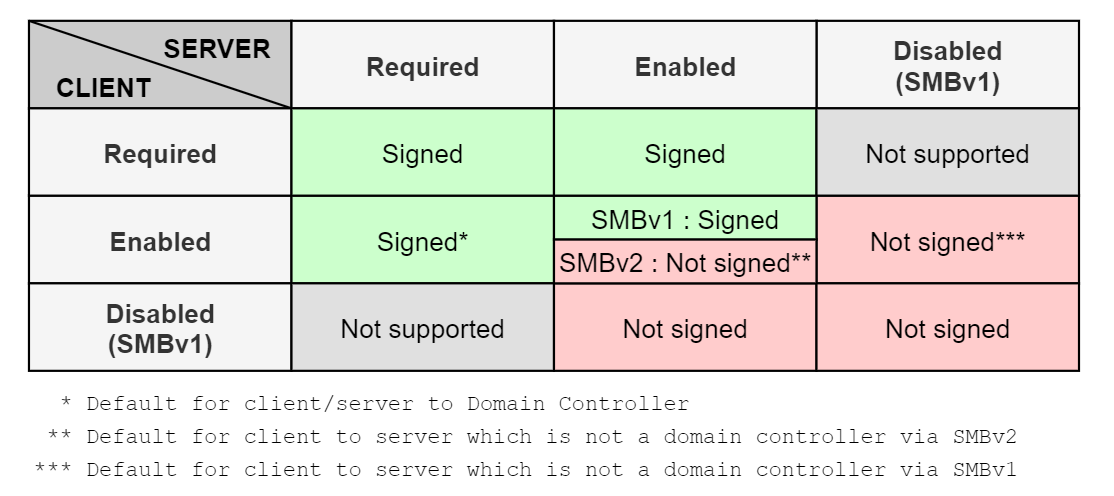
\includegraphics[width=\linewidth]{network/ntlm/images/smb_ntlm_signing_table.png}
  \caption{SMB NTLM signing matrix}
  \label{fig:smb_ntlm_signing_table}
\end{figure}



\subsubsection{LDAP Signature matrix}

For LDAP, there are also three levels:
\begin{itemize}
    \item 
        Disabled: This means that packet signing is not supported.
    \item 
        Negotiated Signing: This option indicates that the machine can handle signing, and if the machine it is communicating with also handles it, then they will be signed.
    \item 
        Required: This finally indicates that signing is not only supported, but that packets must be signed in order for the session to continue.
\end{itemize}


\begin{figure}[!ht]
    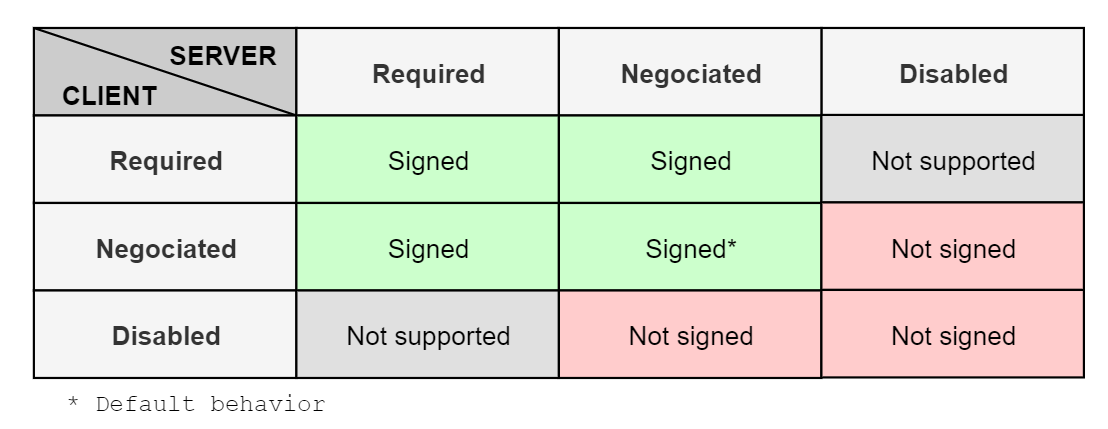
\includegraphics[width=\linewidth]{network/ntlm/images/ldap_ntlm_signing_table.png}
  \caption{LDAP NTLM signing matrix}
  \label{fig:ldap_ntlm_signing_table}
\end{figure}

by default:
\begin{itemize}
    \item all hosts have Negotiated Signing setting. 
    \item the domain controller doesn’t require signing.
\end{itemize}


registry key \verb+ldapserverintegrity+:
\begin{itemize}
    \item DC: \verb+HKLM\System\CurrentControlSet\Services\NTDS\Parameters+
    \item client: \verb+HKLM\System\CurrentControlSet\Services\ldap+
\end{itemize}

value:
\begin{verbatim}
Never       	0
When Supported 	1
Always      	2
\end{verbatim}



\subsection{Authentication signing (MIC)}


The {\bf Message Integrity Code (MIC)} is a signature that is sent only in the last message of an NTLM authentication, the \verb+AUTHENTICATE+ message. It takes into account the 3 messages. The MIC is computed with \verb+HMAC_MD5+ function, using as a key that depends on the client’s secret, called the session key. Therefore, if only one of the 3 messages has been modified, the MIC will no longer be valid, since the concatenation of the 3 messages will not be the same

The MIC can't be removed because there is another flag that indicates that a MIC will be present, \verb+msAvFlags+. It is also present in NTLM response and if it is \verb+0x00000002+, it tells the server that a MIC must be present. So if the server doesn’t see the MIC, it will know that there is something going on, and it will terminate the authentication. If the flag says there must be a MIC, then there must be a MIC.

The \verb+msAcFlags+ can't be reset beacause of the \verb+NTLMv2 Hash+ which is the response to the challenge sent by the server, is a hash that takes into account not only the challenge (obviously), but also all the flags of the response. As you may have guessed, the flag indicating the MIC presence is part of this response.

The MIC protects the integrity of the 3 messages, the \verb+msAvFlags+ protects the presence of the MIC, and the NTLMv2 hash protects the presence of the flag. The attacker, not being aware of the user’s secret, cannot re-compute this hash.

It’s CVE-2019-1040 nicely named Drop the MIC. This vulnerability showed that if the MIC was just removed, even if the flag indicated its presence, the server accepted the authentication without flinching. This was obviously a bug that has since been fixed.

{\bf Drop The MIC 2}


\subsection{Channel Binding / EPA}

This security is built to protect cross-protocol relay.

The principle of this protection is to bind the authentication layer with the protocol in use, even with the TLS layer when it exists (LDAPS or HTTPS for example). The general idea being that in the last NTLM AUTHENTICATE message, a piece of information is put there and cannot be modified by an attacker. This information indicates the desired service, and potentially another information that contains the target server’s certificate’s hash.

\subsubsection{Service binding}

If a client wishes to authenticate to a server to use a specific service, the information identifying the service will be added in the NTLM response. This way, when the legitimate server receives this authentication, it can see the service that was requested by the client, and if it differs from what is actually requested, it will not agree to provide the service.

Since the service namei (SPN) is in the NTLM response, it is protected by the \verb+NtProofStr+ response, which is an \verb+HMAC_MD5+ of this information, the challenge, and other information such as \verb+msAvFlags+. It is computed with the client’s secret.

\subsubsection{TLS binding}

The purpose of this protection is to link the authentication layer, i.e. NTLM messages, to the TLS layer that can potentially be used.

If the client wants to use a protocol encapsulated in TLS (HTTPS, LDAPS for example), it will establish a TLS session with the server, and it will compute the server certificate hash. This hash is called the {\bf Channel Binding Token}, or CBT. Once computed, the client will put this hash in its NTLM response. The legitimate server will then receive the NTLM message at the end of the authentication, read the provided hash, and compare it with the real hash of its certificate. If it is different, it means he wasn’t the original recipient of the NTLM exchange.

Again, since this hash is in the NTLM response, it is protected by the \verb+NtProofStr+ response, like the SPN for Service Binding.

Thanks to this protection, the following two attacks are no longer possible :
\begin{itemize}
    \item  relay information from a client using a protocol without a TLS layer to a protocol with a TLS layer 
    \item relay a protocol with TLS to another protocol with TLS
\end{itemize}


\subsection{Stop. Using. NTLMv1.}

NTLMv2 hash takes into account the server’s challenge, but also the \verb+msAvFlags+ flag which indicates the presence of a MIC field, the field indicating the NetBios name of the target host during authentication, the SPN in case of service binding, and the certificate hash in case of TLS binding.

NTLMv1 protocol doesn’t do that. It only takes into account the server’s challenge. In fact, there is no longer any additional information such as the target name, the \verb+msAvFlags+, the SPN or the CBT.

So, if an NTLMv1 authentication is allowed by a server, an attacker can simply remove the MIC and thus relay authentications to LDAP or LDAPS, for example.

But more importantly, he can make NetLogon requests to retrieve the session key. Indeed, the domain controller has no way to check if he has the right to do so. And since it won’t block a production network that isn’t completely up to date, it will kindly give it to the attacker, for "retro-compatibility reasons".

Once he has the session key, he can sign any packet that he wants. It means that even if the target requests signing, he will be able to do so.

This is by design and it can not be fixed. So I repeat, do not allow NTLMv1 in a production network.
